\documentclass{standalone}
\usepackage{tikz}
\usetikzlibrary{patterns}
\usetikzlibrary{positioning}
\usetikzlibrary{patterns, positioning}
\usetikzlibrary{shapes.misc}
\usepackage[outline]{contour}
\contourlength{1.5pt} 
\usetikzlibrary{calc}
        \usepackage{relsize}
        \tikzset{fontscale/.style = {font=\relsize{#1}}}

\begin{document}
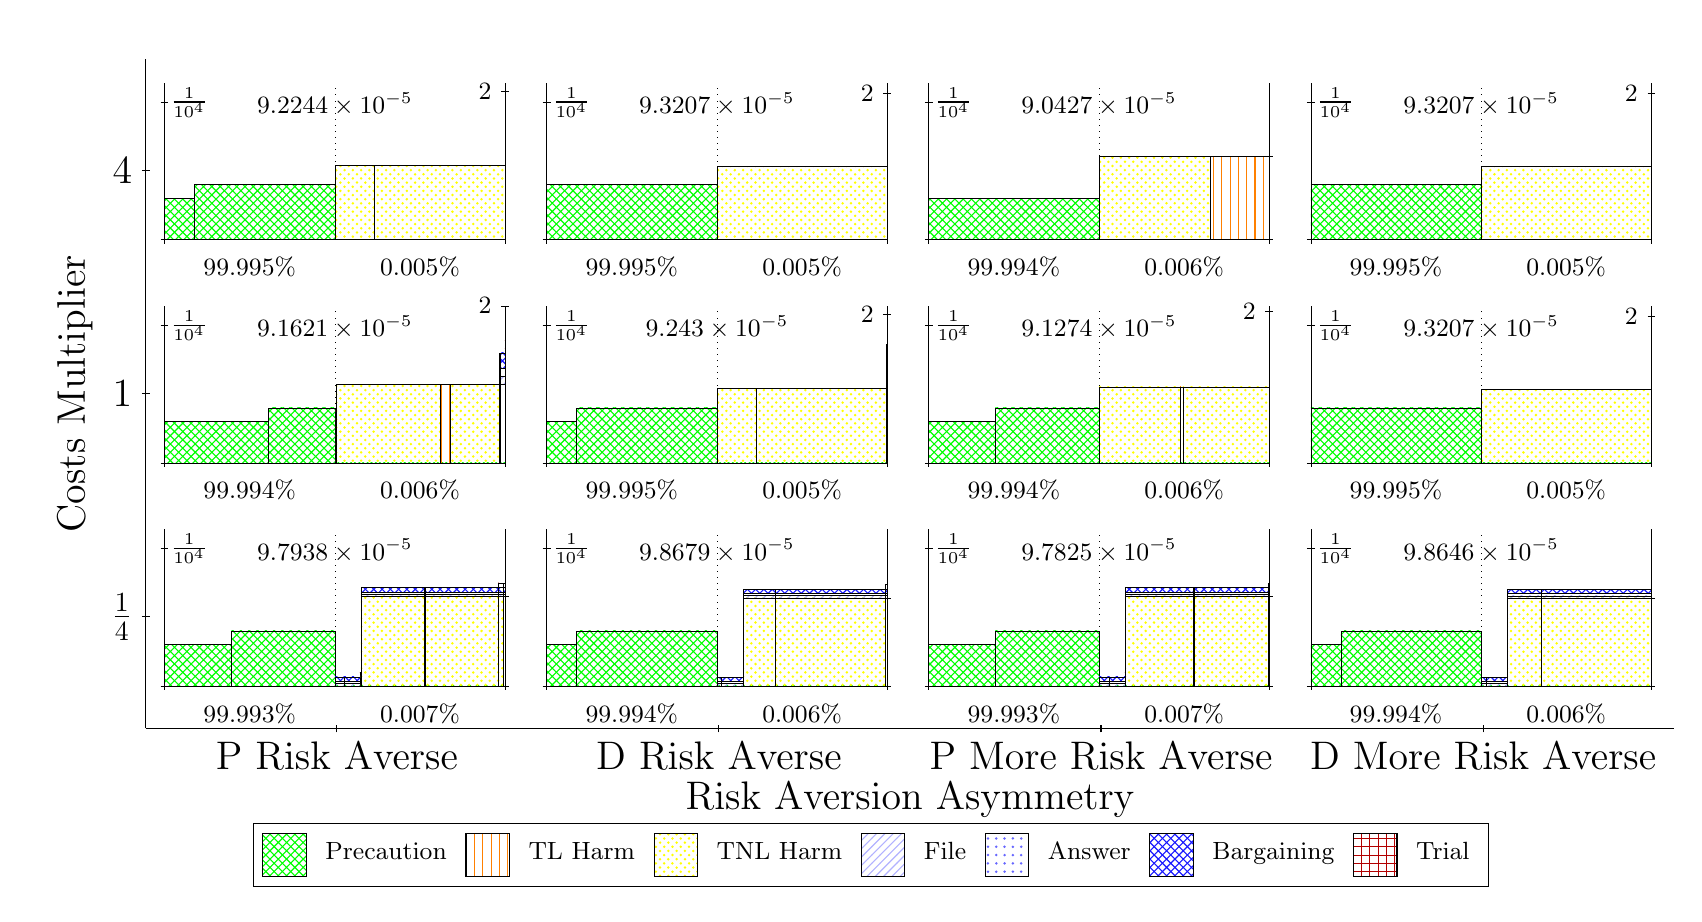
\begin{tikzpicture}
\clip(-0.5,-1.1) rectangle +(20.91,11);
\draw[black] (1,1) -- (1,9.5);
\node[rotate=90, fontscale=2, anchor=center] at (0.1, 5.25) {Costs Multiplier};
\draw[black] (0.95,2.4167) -- (1.05,2.4167);
\node[fontscale=2, anchor=east] at (0.95, 2.4167) {$\frac{1}{4}$};
\draw[black] (0.95,5.25) -- (1.05,5.25);
\node[fontscale=2, anchor=east] at (0.95, 5.25) {1};
\draw[black] (0.95,8.0833) -- (1.05,8.0833);
\node[fontscale=2, anchor=east] at (0.95, 8.0833) {4};

\draw[black] (1,1) -- (20.41,1);
\node[fontscale=2, anchor=center] at (10.705, 0.1) {Risk Aversion Asymmetry};
\draw[black] (3.4263,0.95) -- (3.4263,1.05);
\node[fontscale=2, anchor=north] at (3.4263, 0.95) {P Risk Averse};
\draw[black] (8.2788,0.95) -- (8.2788,1.05);
\node[fontscale=2, anchor=north] at (8.2788, 0.95) {D Risk Averse};
\draw[black] (13.131,0.95) -- (13.131,1.05);
\node[fontscale=2, anchor=north] at (13.131, 0.95) {P More Risk Averse};
\draw[black] (17.984,0.95) -- (17.984,1.05);
\node[fontscale=2, anchor=north] at (17.984, 0.95) {D More Risk Averse};


\draw[pattern=crosshatch, pattern color=green,draw=black,very thin] (1.2381,1.54) rectangle (2.0858,2.0636);
\draw[pattern=crosshatch, pattern color=green,draw=black,very thin] (2.0858,1.54) rectangle (3.4013,2.2381);
\draw[pattern=crosshatch, pattern color=green,draw=black,very thin] (3.4013,1.54) rectangle (3.5176,1.54);
\draw[pattern=north east lines, pattern color=blue!30,draw=black,very thin] (3.4013,1.54) rectangle (3.5176,1.5685);
\draw[pattern=dots,  pattern color=blue!60,draw=black,very thin] (3.4013,1.5685) rectangle (3.5176,1.5969);
\draw[pattern=crosshatch,      pattern color=blue!90,draw=black,very thin] (3.4013,1.5969) rectangle (3.5176,1.6538);
\draw[pattern=crosshatch, pattern color=green,draw=black,very thin] (3.5176,1.54) rectangle (3.7194,1.54);
\draw[pattern=north east lines, pattern color=blue!30,draw=black,very thin] (3.5176,1.54) rectangle (3.7194,1.5685);
\draw[pattern=dots,  pattern color=blue!60,draw=black,very thin] (3.5176,1.5685) rectangle (3.7194,1.5969);
\draw[pattern=crosshatch,      pattern color=blue!90,draw=black,very thin] (3.5176,1.5969) rectangle (3.7194,1.6538);
\draw[pattern=crosshatch, pattern color=green,draw=black,very thin] (3.7194,1.54) rectangle (3.7331,1.54);
\draw[pattern=north east lines, pattern color=blue!30,draw=black,very thin] (3.7194,1.54) rectangle (3.7331,1.5685);
\draw[pattern=dots,  pattern color=blue!60,draw=black,very thin] (3.7194,1.5685) rectangle (3.7331,1.5969);
\draw[pattern=crosshatch,      pattern color=blue!90,draw=black,very thin] (3.7194,1.5969) rectangle (3.7331,1.6538);
\draw[pattern=grid,            pattern color=red!70!black,draw=black,very thin] (3.7194,1.6538) rectangle (3.7331,1.7107);
\draw[pattern=crosshatch, pattern color=green,draw=black,very thin] (3.7331,1.54) rectangle (4.5428,1.54);
\draw[pattern=crosshatch dots, pattern color=yellow,draw=black,very thin] (3.7331,1.54) rectangle (4.5428,2.6779);
\draw[pattern=north east lines, pattern color=blue!30,draw=black,very thin] (3.7331,2.6779) rectangle (4.5428,2.7064);
\draw[pattern=dots,  pattern color=blue!60,draw=black,very thin] (3.7331,2.7064) rectangle (4.5428,2.7348);
\draw[pattern=crosshatch,      pattern color=blue!90,draw=black,very thin] (3.7331,2.7348) rectangle (4.5428,2.7917);
\draw[pattern=crosshatch, pattern color=green,draw=black,very thin] (4.5428,1.54) rectangle (4.5513,1.54);
\draw[pattern=vertical lines, pattern color=orange,draw=black,very thin] (4.5428,1.54) rectangle (4.5513,2.6779);
\draw[pattern=north east lines, pattern color=blue!30,draw=black,very thin] (4.5428,2.6779) rectangle (4.5513,2.7064);
\draw[pattern=dots,  pattern color=blue!60,draw=black,very thin] (4.5428,2.7064) rectangle (4.5513,2.7348);
\draw[pattern=crosshatch,      pattern color=blue!90,draw=black,very thin] (4.5428,2.7348) rectangle (4.5513,2.7917);
\draw[pattern=crosshatch, pattern color=green,draw=black,very thin] (4.5513,1.54) rectangle (5.4823,1.54);
\draw[pattern=crosshatch dots, pattern color=yellow,draw=black,very thin] (4.5513,1.54) rectangle (5.4823,2.6779);
\draw[pattern=north east lines, pattern color=blue!30,draw=black,very thin] (4.5513,2.6779) rectangle (5.4823,2.7064);
\draw[pattern=dots,  pattern color=blue!60,draw=black,very thin] (4.5513,2.7064) rectangle (5.4823,2.7348);
\draw[pattern=crosshatch,      pattern color=blue!90,draw=black,very thin] (4.5513,2.7348) rectangle (5.4823,2.7917);
\draw[pattern=crosshatch, pattern color=green,draw=black,very thin] (5.4823,1.54) rectangle (5.5431,1.54);
\draw[pattern=crosshatch dots, pattern color=yellow,draw=black,very thin] (5.4823,1.54) rectangle (5.5431,2.6779);
\draw[pattern=north east lines, pattern color=blue!30,draw=black,very thin] (5.4823,2.6779) rectangle (5.5431,2.7064);
\draw[pattern=dots,  pattern color=blue!60,draw=black,very thin] (5.4823,2.7064) rectangle (5.5431,2.7348);
\draw[pattern=crosshatch,      pattern color=blue!90,draw=black,very thin] (5.4823,2.7348) rectangle (5.5431,2.7917);
\draw[pattern=grid,            pattern color=red!70!black,draw=black,very thin] (5.4823,2.7917) rectangle (5.5431,2.8486);
\draw[pattern=crosshatch, pattern color=green,draw=black,very thin] (5.5431,1.54) rectangle (5.5644,1.54);
\draw[pattern=vertical lines, pattern color=orange,draw=black,very thin] (5.5431,1.54) rectangle (5.5644,2.6779);
\draw[pattern=north east lines, pattern color=blue!30,draw=black,very thin] (5.5431,2.6779) rectangle (5.5644,2.7064);
\draw[pattern=dots,  pattern color=blue!60,draw=black,very thin] (5.5431,2.7064) rectangle (5.5644,2.7348);
\draw[pattern=crosshatch,      pattern color=blue!90,draw=black,very thin] (5.5431,2.7348) rectangle (5.5644,2.7917);
\draw[pattern=grid,            pattern color=red!70!black,draw=black,very thin] (5.5431,2.7917) rectangle (5.5644,2.8486);
\node[font=\small,text=black,anchor=north] at (3.4013, 3.5333) {$9.7938\times 10^{-5}$};
\draw[black,very thin] (1.2381,1.54) -- (1.2381,3.5333);
\draw[black,very thin] (1.1881,1.54) -- (1.2881,1.54);
\node[font=\small,text=black, anchor=west] at (1.1881, 1.54) {};
\draw[black,very thin] (1.1881,3.2853) -- (1.2881,3.2853);
\node[font=\small,text=black, anchor=west] at (1.1881, 3.2853) {$\frac{1}{10^{4}}$};

\draw[black,dotted,very thin] (3.4013,1.5998) -- (3.4013,3.4735);
\draw[black,very thin] (5.5644,1.54) -- (5.5644,3.5333);
\draw[black,very thin] (5.5144,1.54) -- (5.6144,1.54);
\node[font=\small,text=black, anchor=east] at (5.5144, 1.54) {\contour{white}{}};
\draw[black,very thin] (5.5144,2.6779) -- (5.6144,2.6779);
\node[font=\small,text=black, anchor=east] at (5.5144, 2.6779) {\contour{white}{}};

\draw[black,very thin] (1.2381,1.54) -- (5.5644,1.54);
\draw[black,very thin] (1.2381,1.49) -- (1.2381,1.59);
\node[font=\small,text=black, anchor=north] at (1.2381, 1.49) {};
\draw[black,very thin] (5.5644,1.49) -- (5.5644,1.59);
\node[font=\small,text=black, anchor=north] at (5.5644, 1.49) {};

\node[font=\small,text=black,anchor=south] at (2.3197, 0.94) {99.993\%};
\node[font=\small,text=black,anchor=south] at (4.4828, 0.94) {0.007\%};

\draw[pattern=crosshatch, pattern color=green,draw=black,very thin] (6.0906,1.54) rectangle (6.4717,2.0636);
\draw[pattern=crosshatch, pattern color=green,draw=black,very thin] (6.4717,1.54) rectangle (8.2538,2.2381);
\draw[pattern=crosshatch, pattern color=green,draw=black,very thin] (8.2538,1.54) rectangle (8.3101,1.54);
\draw[pattern=north east lines, pattern color=blue!30,draw=black,very thin] (8.2538,1.54) rectangle (8.3101,1.568);
\draw[pattern=dots,  pattern color=blue!60,draw=black,very thin] (8.2538,1.568) rectangle (8.3101,1.5959);
\draw[pattern=crosshatch,      pattern color=blue!90,draw=black,very thin] (8.2538,1.5959) rectangle (8.3101,1.6518);
\draw[pattern=crosshatch, pattern color=green,draw=black,very thin] (8.3101,1.54) rectangle (8.5885,1.54);
\draw[pattern=north east lines, pattern color=blue!30,draw=black,very thin] (8.3101,1.54) rectangle (8.5885,1.568);
\draw[pattern=dots,  pattern color=blue!60,draw=black,very thin] (8.3101,1.568) rectangle (8.5885,1.5959);
\draw[pattern=crosshatch,      pattern color=blue!90,draw=black,very thin] (8.3101,1.5959) rectangle (8.5885,1.6518);
\draw[pattern=crosshatch, pattern color=green,draw=black,very thin] (8.5885,1.54) rectangle (8.5917,1.54);
\draw[pattern=north east lines, pattern color=blue!30,draw=black,very thin] (8.5885,1.54) rectangle (8.5917,1.568);
\draw[pattern=dots,  pattern color=blue!60,draw=black,very thin] (8.5885,1.568) rectangle (8.5917,1.5959);
\draw[pattern=crosshatch,      pattern color=blue!90,draw=black,very thin] (8.5885,1.5959) rectangle (8.5917,1.6518);
\draw[pattern=grid,            pattern color=red!70!black,draw=black,very thin] (8.5885,1.6518) rectangle (8.5917,1.7076);
\draw[pattern=crosshatch, pattern color=green,draw=black,very thin] (8.5917,1.54) rectangle (8.9977,1.54);
\draw[pattern=crosshatch dots, pattern color=yellow,draw=black,very thin] (8.5917,1.54) rectangle (8.9977,2.6572);
\draw[pattern=north east lines, pattern color=blue!30,draw=black,very thin] (8.5917,2.6572) rectangle (8.9977,2.6851);
\draw[pattern=dots,  pattern color=blue!60,draw=black,very thin] (8.5917,2.6851) rectangle (8.9977,2.7131);
\draw[pattern=crosshatch,      pattern color=blue!90,draw=black,very thin] (8.5917,2.7131) rectangle (8.9977,2.7689);
\draw[pattern=crosshatch, pattern color=green,draw=black,very thin] (8.9977,1.54) rectangle (8.9984,1.54);
\draw[pattern=vertical lines, pattern color=orange,draw=black,very thin] (8.9977,1.54) rectangle (8.9984,2.6572);
\draw[pattern=north east lines, pattern color=blue!30,draw=black,very thin] (8.9977,2.6572) rectangle (8.9984,2.6851);
\draw[pattern=dots,  pattern color=blue!60,draw=black,very thin] (8.9977,2.6851) rectangle (8.9984,2.7131);
\draw[pattern=crosshatch,      pattern color=blue!90,draw=black,very thin] (8.9977,2.7131) rectangle (8.9984,2.7689);
\draw[pattern=crosshatch, pattern color=green,draw=black,very thin] (8.9984,1.54) rectangle (10.397,1.54);
\draw[pattern=crosshatch dots, pattern color=yellow,draw=black,very thin] (8.9984,1.54) rectangle (10.397,2.6572);
\draw[pattern=north east lines, pattern color=blue!30,draw=black,very thin] (8.9984,2.6572) rectangle (10.397,2.6851);
\draw[pattern=dots,  pattern color=blue!60,draw=black,very thin] (8.9984,2.6851) rectangle (10.397,2.7131);
\draw[pattern=crosshatch,      pattern color=blue!90,draw=black,very thin] (8.9984,2.7131) rectangle (10.397,2.7689);
\draw[pattern=crosshatch, pattern color=green,draw=black,very thin] (10.397,1.54) rectangle (10.415,1.54);
\draw[pattern=crosshatch dots, pattern color=yellow,draw=black,very thin] (10.397,1.54) rectangle (10.415,2.6572);
\draw[pattern=north east lines, pattern color=blue!30,draw=black,very thin] (10.397,2.6572) rectangle (10.415,2.6851);
\draw[pattern=dots,  pattern color=blue!60,draw=black,very thin] (10.397,2.6851) rectangle (10.415,2.7131);
\draw[pattern=crosshatch,      pattern color=blue!90,draw=black,very thin] (10.397,2.7131) rectangle (10.415,2.7689);
\draw[pattern=grid,            pattern color=red!70!black,draw=black,very thin] (10.397,2.7689) rectangle (10.415,2.8248);
\draw[pattern=crosshatch, pattern color=green,draw=black,very thin] (10.415,1.54) rectangle (10.417,1.54);
\draw[pattern=vertical lines, pattern color=orange,draw=black,very thin] (10.415,1.54) rectangle (10.417,2.6572);
\draw[pattern=north east lines, pattern color=blue!30,draw=black,very thin] (10.415,2.6572) rectangle (10.417,2.6851);
\draw[pattern=dots,  pattern color=blue!60,draw=black,very thin] (10.415,2.6851) rectangle (10.417,2.7131);
\draw[pattern=crosshatch,      pattern color=blue!90,draw=black,very thin] (10.415,2.7131) rectangle (10.417,2.7689);
\draw[pattern=grid,            pattern color=red!70!black,draw=black,very thin] (10.415,2.7689) rectangle (10.417,2.8248);
\node[font=\small,text=black,anchor=north] at (8.2538, 3.5333) {$9.8679\times 10^{-5}$};
\draw[black,very thin] (6.0906,1.54) -- (6.0906,3.5333);
\draw[black,very thin] (6.0406,1.54) -- (6.1406,1.54);
\node[font=\small,text=black, anchor=west] at (6.0406, 1.54) {};
\draw[black,very thin] (6.0406,3.2853) -- (6.1406,3.2853);
\node[font=\small,text=black, anchor=west] at (6.0406, 3.2853) {$\frac{1}{10^{4}}$};

\draw[black,dotted,very thin] (8.2538,1.5998) -- (8.2538,3.4735);
\draw[black,very thin] (10.417,1.54) -- (10.417,3.5333);
\draw[black,very thin] (10.367,1.54) -- (10.467,1.54);
\node[font=\small,text=black, anchor=east] at (10.367, 1.54) {\contour{white}{}};
\draw[black,very thin] (10.367,2.6572) -- (10.467,2.6572);
\node[font=\small,text=black, anchor=east] at (10.367, 2.6572) {\contour{white}{}};

\draw[black,very thin] (6.0906,1.54) -- (10.417,1.54);
\draw[black,very thin] (6.0906,1.49) -- (6.0906,1.59);
\node[font=\small,text=black, anchor=north] at (6.0906, 1.49) {};
\draw[black,very thin] (10.417,1.49) -- (10.417,1.59);
\node[font=\small,text=black, anchor=north] at (10.417, 1.49) {};

\node[font=\small,text=black,anchor=south] at (7.1722, 0.94) {99.994\%};
\node[font=\small,text=black,anchor=south] at (9.3353, 0.94) {0.006\%};

\draw[pattern=crosshatch, pattern color=green,draw=black,very thin] (10.943,1.54) rectangle (11.791,2.0636);
\draw[pattern=crosshatch, pattern color=green,draw=black,very thin] (11.791,1.54) rectangle (13.106,2.2381);
\draw[pattern=crosshatch, pattern color=green,draw=black,very thin] (13.106,1.54) rectangle (13.233,1.54);
\draw[pattern=north east lines, pattern color=blue!30,draw=black,very thin] (13.106,1.54) rectangle (13.233,1.5685);
\draw[pattern=dots,  pattern color=blue!60,draw=black,very thin] (13.106,1.5685) rectangle (13.233,1.5969);
\draw[pattern=crosshatch,      pattern color=blue!90,draw=black,very thin] (13.106,1.5969) rectangle (13.233,1.6538);
\draw[pattern=crosshatch, pattern color=green,draw=black,very thin] (13.233,1.54) rectangle (13.435,1.54);
\draw[pattern=north east lines, pattern color=blue!30,draw=black,very thin] (13.233,1.54) rectangle (13.435,1.5685);
\draw[pattern=dots,  pattern color=blue!60,draw=black,very thin] (13.233,1.5685) rectangle (13.435,1.5969);
\draw[pattern=crosshatch,      pattern color=blue!90,draw=black,very thin] (13.233,1.5969) rectangle (13.435,1.6538);
\draw[pattern=crosshatch, pattern color=green,draw=black,very thin] (13.435,1.54) rectangle (13.438,1.54);
\draw[pattern=north east lines, pattern color=blue!30,draw=black,very thin] (13.435,1.54) rectangle (13.438,1.5685);
\draw[pattern=dots,  pattern color=blue!60,draw=black,very thin] (13.435,1.5685) rectangle (13.438,1.5969);
\draw[pattern=crosshatch,      pattern color=blue!90,draw=black,very thin] (13.435,1.5969) rectangle (13.438,1.6538);
\draw[pattern=grid,            pattern color=red!70!black,draw=black,very thin] (13.435,1.6538) rectangle (13.438,1.7107);
\draw[pattern=crosshatch, pattern color=green,draw=black,very thin] (13.438,1.54) rectangle (14.3,1.54);
\draw[pattern=crosshatch dots, pattern color=yellow,draw=black,very thin] (13.438,1.54) rectangle (14.3,2.6779);
\draw[pattern=north east lines, pattern color=blue!30,draw=black,very thin] (13.438,2.6779) rectangle (14.3,2.7064);
\draw[pattern=dots,  pattern color=blue!60,draw=black,very thin] (13.438,2.7064) rectangle (14.3,2.7348);
\draw[pattern=crosshatch,      pattern color=blue!90,draw=black,very thin] (13.438,2.7348) rectangle (14.3,2.7917);
\draw[pattern=crosshatch, pattern color=green,draw=black,very thin] (14.3,1.54) rectangle (14.321,1.54);
\draw[pattern=vertical lines, pattern color=orange,draw=black,very thin] (14.3,1.54) rectangle (14.321,2.6779);
\draw[pattern=north east lines, pattern color=blue!30,draw=black,very thin] (14.3,2.6779) rectangle (14.321,2.7064);
\draw[pattern=dots,  pattern color=blue!60,draw=black,very thin] (14.3,2.7064) rectangle (14.321,2.7348);
\draw[pattern=crosshatch,      pattern color=blue!90,draw=black,very thin] (14.3,2.7348) rectangle (14.321,2.7917);
\draw[pattern=crosshatch, pattern color=green,draw=black,very thin] (14.321,1.54) rectangle (15.252,1.54);
\draw[pattern=crosshatch dots, pattern color=yellow,draw=black,very thin] (14.321,1.54) rectangle (15.252,2.6779);
\draw[pattern=north east lines, pattern color=blue!30,draw=black,very thin] (14.321,2.6779) rectangle (15.252,2.7064);
\draw[pattern=dots,  pattern color=blue!60,draw=black,very thin] (14.321,2.7064) rectangle (15.252,2.7348);
\draw[pattern=crosshatch,      pattern color=blue!90,draw=black,very thin] (14.321,2.7348) rectangle (15.252,2.7917);
\draw[pattern=crosshatch, pattern color=green,draw=black,very thin] (15.252,1.54) rectangle (15.261,1.54);
\draw[pattern=crosshatch dots, pattern color=yellow,draw=black,very thin] (15.252,1.54) rectangle (15.261,2.6779);
\draw[pattern=north east lines, pattern color=blue!30,draw=black,very thin] (15.252,2.6779) rectangle (15.261,2.7064);
\draw[pattern=dots,  pattern color=blue!60,draw=black,very thin] (15.252,2.7064) rectangle (15.261,2.7348);
\draw[pattern=crosshatch,      pattern color=blue!90,draw=black,very thin] (15.252,2.7348) rectangle (15.261,2.7917);
\draw[pattern=grid,            pattern color=red!70!black,draw=black,very thin] (15.252,2.7917) rectangle (15.261,2.8486);
\draw[pattern=crosshatch, pattern color=green,draw=black,very thin] (15.261,1.54) rectangle (15.269,1.54);
\draw[pattern=vertical lines, pattern color=orange,draw=black,very thin] (15.261,1.54) rectangle (15.269,2.6779);
\draw[pattern=north east lines, pattern color=blue!30,draw=black,very thin] (15.261,2.6779) rectangle (15.269,2.7064);
\draw[pattern=dots,  pattern color=blue!60,draw=black,very thin] (15.261,2.7064) rectangle (15.269,2.7348);
\draw[pattern=crosshatch,      pattern color=blue!90,draw=black,very thin] (15.261,2.7348) rectangle (15.269,2.7917);
\draw[pattern=grid,            pattern color=red!70!black,draw=black,very thin] (15.261,2.7917) rectangle (15.269,2.8486);
\node[font=\small,text=black,anchor=north] at (13.106, 3.5333) {$9.7825\times 10^{-5}$};
\draw[black,very thin] (10.943,1.54) -- (10.943,3.5333);
\draw[black,very thin] (10.893,1.54) -- (10.993,1.54);
\node[font=\small,text=black, anchor=west] at (10.893, 1.54) {};
\draw[black,very thin] (10.893,3.2853) -- (10.993,3.2853);
\node[font=\small,text=black, anchor=west] at (10.893, 3.2853) {$\frac{1}{10^{4}}$};

\draw[black,dotted,very thin] (13.106,1.5998) -- (13.106,3.4735);
\draw[black,very thin] (15.269,1.54) -- (15.269,3.5333);
\draw[black,very thin] (15.219,1.54) -- (15.319,1.54);
\node[font=\small,text=black, anchor=east] at (15.219, 1.54) {\contour{white}{}};
\draw[black,very thin] (15.219,2.6779) -- (15.319,2.6779);
\node[font=\small,text=black, anchor=east] at (15.219, 2.6779) {\contour{white}{}};

\draw[black,very thin] (10.943,1.54) -- (15.269,1.54);
\draw[black,very thin] (10.943,1.49) -- (10.943,1.59);
\node[font=\small,text=black, anchor=north] at (10.943, 1.49) {};
\draw[black,very thin] (15.269,1.49) -- (15.269,1.59);
\node[font=\small,text=black, anchor=north] at (15.269, 1.49) {};

\node[font=\small,text=black,anchor=south] at (12.025, 0.94) {99.993\%};
\node[font=\small,text=black,anchor=south] at (14.188, 0.94) {0.007\%};

\draw[pattern=crosshatch, pattern color=green,draw=black,very thin] (15.796,1.54) rectangle (16.177,2.0636);
\draw[pattern=crosshatch, pattern color=green,draw=black,very thin] (16.177,1.54) rectangle (17.959,2.2381);
\draw[pattern=crosshatch, pattern color=green,draw=black,very thin] (17.959,1.54) rectangle (18.018,1.54);
\draw[pattern=north east lines, pattern color=blue!30,draw=black,very thin] (17.959,1.54) rectangle (18.018,1.568);
\draw[pattern=dots,  pattern color=blue!60,draw=black,very thin] (17.959,1.568) rectangle (18.018,1.5959);
\draw[pattern=crosshatch,      pattern color=blue!90,draw=black,very thin] (17.959,1.5959) rectangle (18.018,1.6517);
\draw[pattern=crosshatch, pattern color=green,draw=black,very thin] (18.018,1.54) rectangle (18.296,1.54);
\draw[pattern=north east lines, pattern color=blue!30,draw=black,very thin] (18.018,1.54) rectangle (18.296,1.568);
\draw[pattern=dots,  pattern color=blue!60,draw=black,very thin] (18.018,1.568) rectangle (18.296,1.5959);
\draw[pattern=crosshatch,      pattern color=blue!90,draw=black,very thin] (18.018,1.5959) rectangle (18.296,1.6517);
\draw[pattern=crosshatch, pattern color=green,draw=black,very thin] (18.296,1.54) rectangle (18.719,1.54);
\draw[pattern=crosshatch dots, pattern color=yellow,draw=black,very thin] (18.296,1.54) rectangle (18.719,2.6569);
\draw[pattern=north east lines, pattern color=blue!30,draw=black,very thin] (18.296,2.6569) rectangle (18.719,2.6848);
\draw[pattern=dots,  pattern color=blue!60,draw=black,very thin] (18.296,2.6848) rectangle (18.719,2.7128);
\draw[pattern=crosshatch,      pattern color=blue!90,draw=black,very thin] (18.296,2.7128) rectangle (18.719,2.7686);
\draw[pattern=crosshatch, pattern color=green,draw=black,very thin] (18.719,1.54) rectangle (18.72,1.54);
\draw[pattern=vertical lines, pattern color=orange,draw=black,very thin] (18.719,1.54) rectangle (18.72,2.6569);
\draw[pattern=north east lines, pattern color=blue!30,draw=black,very thin] (18.719,2.6569) rectangle (18.72,2.6848);
\draw[pattern=dots,  pattern color=blue!60,draw=black,very thin] (18.719,2.6848) rectangle (18.72,2.7128);
\draw[pattern=crosshatch,      pattern color=blue!90,draw=black,very thin] (18.719,2.7128) rectangle (18.72,2.7686);
\draw[pattern=crosshatch, pattern color=green,draw=black,very thin] (18.72,1.54) rectangle (20.119,1.54);
\draw[pattern=crosshatch dots, pattern color=yellow,draw=black,very thin] (18.72,1.54) rectangle (20.119,2.6569);
\draw[pattern=north east lines, pattern color=blue!30,draw=black,very thin] (18.72,2.6569) rectangle (20.119,2.6849);
\draw[pattern=dots,  pattern color=blue!60,draw=black,very thin] (18.72,2.6849) rectangle (20.119,2.7128);
\draw[pattern=crosshatch,      pattern color=blue!90,draw=black,very thin] (18.72,2.7128) rectangle (20.119,2.7686);
\draw[pattern=crosshatch, pattern color=green,draw=black,very thin] (20.119,1.54) rectangle (20.121,1.54);
\draw[pattern=crosshatch dots, pattern color=yellow,draw=black,very thin] (20.119,1.54) rectangle (20.121,2.6569);
\draw[pattern=north east lines, pattern color=blue!30,draw=black,very thin] (20.119,2.6569) rectangle (20.121,2.6848);
\draw[pattern=dots,  pattern color=blue!60,draw=black,very thin] (20.119,2.6848) rectangle (20.121,2.7128);
\draw[pattern=crosshatch,      pattern color=blue!90,draw=black,very thin] (20.119,2.7128) rectangle (20.121,2.7686);
\draw[pattern=grid,            pattern color=red!70!black,draw=black,very thin] (20.119,2.7686) rectangle (20.121,2.8245);
\draw[pattern=crosshatch, pattern color=green,draw=black,very thin] (20.121,1.54) rectangle (20.122,1.54);
\draw[pattern=vertical lines, pattern color=orange,draw=black,very thin] (20.121,1.54) rectangle (20.122,2.6569);
\draw[pattern=north east lines, pattern color=blue!30,draw=black,very thin] (20.121,2.6569) rectangle (20.122,2.6848);
\draw[pattern=dots,  pattern color=blue!60,draw=black,very thin] (20.121,2.6848) rectangle (20.122,2.7128);
\draw[pattern=crosshatch,      pattern color=blue!90,draw=black,very thin] (20.121,2.7128) rectangle (20.122,2.7686);
\draw[pattern=grid,            pattern color=red!70!black,draw=black,very thin] (20.121,2.7686) rectangle (20.122,2.8245);
\node[font=\small,text=black,anchor=north] at (17.959, 3.5333) {$9.8646\times 10^{-5}$};
\draw[black,very thin] (15.796,1.54) -- (15.796,3.5333);
\draw[black,very thin] (15.746,1.54) -- (15.846,1.54);
\node[font=\small,text=black, anchor=west] at (15.746, 1.54) {};
\draw[black,very thin] (15.746,3.2853) -- (15.846,3.2853);
\node[font=\small,text=black, anchor=west] at (15.746, 3.2853) {$\frac{1}{10^{4}}$};

\draw[black,dotted,very thin] (17.959,1.5998) -- (17.959,3.4735);
\draw[black,very thin] (20.122,1.54) -- (20.122,3.5333);
\draw[black,very thin] (20.072,1.54) -- (20.172,1.54);
\node[font=\small,text=black, anchor=east] at (20.072, 1.54) {\contour{white}{}};
\draw[black,very thin] (20.072,2.6569) -- (20.172,2.6569);
\node[font=\small,text=black, anchor=east] at (20.072, 2.6569) {\contour{white}{}};

\draw[black,very thin] (15.796,1.54) -- (20.122,1.54);
\draw[black,very thin] (15.796,1.49) -- (15.796,1.59);
\node[font=\small,text=black, anchor=north] at (15.796, 1.49) {};
\draw[black,very thin] (20.122,1.49) -- (20.122,1.59);
\node[font=\small,text=black, anchor=north] at (20.122, 1.49) {};

\node[font=\small,text=black,anchor=south] at (16.877, 0.94) {99.994\%};
\node[font=\small,text=black,anchor=south] at (19.04, 0.94) {0.006\%};

\draw[pattern=crosshatch, pattern color=green,draw=black,very thin] (1.2381,4.3733) rectangle (2.5535,4.8969);
\draw[pattern=crosshatch, pattern color=green,draw=black,very thin] (2.5535,4.3733) rectangle (3.4013,5.0715);
\draw[pattern=crosshatch, pattern color=green,draw=black,very thin] (3.4013,4.3733) rectangle (3.4149,4.3734);
\draw[pattern=north east lines, pattern color=blue!30,draw=black,very thin] (3.4013,4.3734) rectangle (3.4149,4.473);
\draw[pattern=dots,  pattern color=blue!60,draw=black,very thin] (3.4013,4.473) rectangle (3.4149,4.5727);
\draw[pattern=crosshatch,      pattern color=blue!90,draw=black,very thin] (3.4013,4.5727) rectangle (3.4149,4.772);
\draw[pattern=crosshatch, pattern color=green,draw=black,very thin] (3.4149,4.3733) rectangle (4.7369,4.3734);
\draw[pattern=crosshatch dots, pattern color=yellow,draw=black,very thin] (3.4149,4.3734) rectangle (4.7369,5.37);
\draw[pattern=crosshatch, pattern color=green,draw=black,very thin] (4.7369,4.3733) rectangle (4.8607,4.3734);
\draw[pattern=vertical lines, pattern color=orange,draw=black,very thin] (4.7369,4.3734) rectangle (4.8607,5.37);
\draw[pattern=crosshatch, pattern color=green,draw=black,very thin] (4.8607,4.3733) rectangle (5.4886,4.3734);
\draw[pattern=crosshatch dots, pattern color=yellow,draw=black,very thin] (4.8607,4.3734) rectangle (5.4886,5.37);
\draw[pattern=crosshatch, pattern color=green,draw=black,very thin] (5.4886,4.3733) rectangle (5.5049,4.3734);
\draw[pattern=crosshatch dots, pattern color=yellow,draw=black,very thin] (5.4886,4.3734) rectangle (5.5049,5.37);
\draw[pattern=north east lines, pattern color=blue!30,draw=black,very thin] (5.4886,5.37) rectangle (5.5049,5.4697);
\draw[pattern=dots,  pattern color=blue!60,draw=black,very thin] (5.4886,5.4697) rectangle (5.5049,5.5693);
\draw[pattern=crosshatch,      pattern color=blue!90,draw=black,very thin] (5.4886,5.5693) rectangle (5.5049,5.7687);
\draw[pattern=crosshatch, pattern color=green,draw=black,very thin] (5.5049,4.3733) rectangle (5.561,4.3734);
\draw[pattern=vertical lines, pattern color=orange,draw=black,very thin] (5.5049,4.3734) rectangle (5.561,5.37);
\draw[pattern=north east lines, pattern color=blue!30,draw=black,very thin] (5.5049,5.37) rectangle (5.561,5.4697);
\draw[pattern=dots,  pattern color=blue!60,draw=black,very thin] (5.5049,5.4697) rectangle (5.561,5.5693);
\draw[pattern=crosshatch,      pattern color=blue!90,draw=black,very thin] (5.5049,5.5693) rectangle (5.561,5.7687);
\draw[pattern=crosshatch, pattern color=green,draw=black,very thin] (5.561,4.3733) rectangle (5.5636,4.3734);
\draw[pattern=crosshatch dots, pattern color=yellow,draw=black,very thin] (5.561,4.3734) rectangle (5.5636,5.37);
\draw[pattern=north east lines, pattern color=blue!30,draw=black,very thin] (5.561,5.37) rectangle (5.5636,5.4697);
\draw[pattern=dots,  pattern color=blue!60,draw=black,very thin] (5.561,5.4697) rectangle (5.5636,5.5693);
\draw[pattern=crosshatch,      pattern color=blue!90,draw=black,very thin] (5.561,5.5693) rectangle (5.5636,5.7687);
\draw[pattern=grid,            pattern color=red!70!black,draw=black,very thin] (5.561,5.7687) rectangle (5.5636,5.968);
\draw[pattern=crosshatch, pattern color=green,draw=black,very thin] (5.5636,4.3733) rectangle (5.5644,4.3734);
\draw[pattern=vertical lines, pattern color=orange,draw=black,very thin] (5.5636,4.3734) rectangle (5.5644,5.37);
\draw[pattern=north east lines, pattern color=blue!30,draw=black,very thin] (5.5636,5.37) rectangle (5.5644,5.4697);
\draw[pattern=dots,  pattern color=blue!60,draw=black,very thin] (5.5636,5.4697) rectangle (5.5644,5.5693);
\draw[pattern=crosshatch,      pattern color=blue!90,draw=black,very thin] (5.5636,5.5693) rectangle (5.5644,5.7687);
\draw[pattern=grid,            pattern color=red!70!black,draw=black,very thin] (5.5636,5.7687) rectangle (5.5644,5.968);
\node[font=\small,text=black,anchor=north] at (3.4013, 6.3667) {$9.1621\times 10^{-5}$};
\draw[black,very thin] (1.2381,4.3733) -- (1.2381,6.3667);
\draw[black,very thin] (1.1881,4.3733) -- (1.2881,4.3733);
\node[font=\small,text=black, anchor=west] at (1.1881, 4.3733) {};
\draw[black,very thin] (1.1881,6.1186) -- (1.2881,6.1186);
\node[font=\small,text=black, anchor=west] at (1.1881, 6.1186) {$\frac{1}{10^{4}}$};

\draw[black,dotted,very thin] (3.4013,4.4331) -- (3.4013,6.3069);
\draw[black,very thin] (5.5644,4.3733) -- (5.5644,6.3667);
\draw[black,very thin] (5.5144,6.3666) -- (5.6144,6.3666);
\node[font=\small,text=black, anchor=east] at (5.5144, 6.3666) {\contour{white}{2}};

\draw[black,very thin] (1.2381,4.3733) -- (5.5644,4.3733);
\draw[black,very thin] (1.2381,4.3233) -- (1.2381,4.4233);
\node[font=\small,text=black, anchor=north] at (1.2381, 4.3233) {};
\draw[black,very thin] (5.5644,4.3233) -- (5.5644,4.4233);
\node[font=\small,text=black, anchor=north] at (5.5644, 4.3233) {};

\node[font=\small,text=black,anchor=south] at (2.3197, 3.7733) {99.994\%};
\node[font=\small,text=black,anchor=south] at (4.4828, 3.7733) {0.006\%};

\draw[pattern=crosshatch, pattern color=green,draw=black,very thin] (6.0906,4.3733) rectangle (6.4717,4.8969);
\draw[pattern=crosshatch, pattern color=green,draw=black,very thin] (6.4717,4.3733) rectangle (8.2538,5.0715);
\draw[pattern=crosshatch, pattern color=green,draw=black,very thin] (8.2538,4.3733) rectangle (8.2555,4.3734);
\draw[pattern=north east lines, pattern color=blue!30,draw=black,very thin] (8.2538,4.3734) rectangle (8.2555,4.4677);
\draw[pattern=dots,  pattern color=blue!60,draw=black,very thin] (8.2538,4.4677) rectangle (8.2555,4.562);
\draw[pattern=crosshatch,      pattern color=blue!90,draw=black,very thin] (8.2538,4.562) rectangle (8.2555,4.7507);
\draw[pattern=grid,            pattern color=red!70!black,draw=black,very thin] (8.2538,4.7507) rectangle (8.2555,4.9394);
\draw[pattern=crosshatch, pattern color=green,draw=black,very thin] (8.2555,4.3733) rectangle (8.7486,4.3734);
\draw[pattern=crosshatch dots, pattern color=yellow,draw=black,very thin] (8.2555,4.3734) rectangle (8.7486,5.3167);
\draw[pattern=crosshatch, pattern color=green,draw=black,very thin] (8.7486,4.3733) rectangle (8.7502,4.3734);
\draw[pattern=vertical lines, pattern color=orange,draw=black,very thin] (8.7486,4.3734) rectangle (8.7502,5.3167);
\draw[pattern=crosshatch, pattern color=green,draw=black,very thin] (8.7502,4.3733) rectangle (10.406,4.3734);
\draw[pattern=crosshatch dots, pattern color=yellow,draw=black,very thin] (8.7502,4.3734) rectangle (10.406,5.3167);
\draw[pattern=crosshatch, pattern color=green,draw=black,very thin] (10.406,4.3733) rectangle (10.416,4.3734);
\draw[pattern=crosshatch dots, pattern color=yellow,draw=black,very thin] (10.406,4.3734) rectangle (10.416,5.3167);
\draw[pattern=north east lines, pattern color=blue!30,draw=black,very thin] (10.406,5.3167) rectangle (10.416,5.4111);
\draw[pattern=dots,  pattern color=blue!60,draw=black,very thin] (10.406,5.4111) rectangle (10.416,5.5054);
\draw[pattern=crosshatch,      pattern color=blue!90,draw=black,very thin] (10.406,5.5054) rectangle (10.416,5.6941);
\draw[pattern=grid,            pattern color=red!70!black,draw=black,very thin] (10.406,5.6941) rectangle (10.416,5.8827);
\draw[pattern=crosshatch, pattern color=green,draw=black,very thin] (10.416,4.3733) rectangle (10.417,4.3734);
\draw[pattern=vertical lines, pattern color=orange,draw=black,very thin] (10.416,4.3734) rectangle (10.417,5.3167);
\draw[pattern=north east lines, pattern color=blue!30,draw=black,very thin] (10.416,5.3167) rectangle (10.417,5.4111);
\draw[pattern=dots,  pattern color=blue!60,draw=black,very thin] (10.416,5.4111) rectangle (10.417,5.5054);
\draw[pattern=crosshatch,      pattern color=blue!90,draw=black,very thin] (10.416,5.5054) rectangle (10.417,5.6941);
\draw[pattern=grid,            pattern color=red!70!black,draw=black,very thin] (10.416,5.6941) rectangle (10.417,5.8827);
\node[font=\small,text=black,anchor=north] at (8.2538, 6.3667) {$9.243\times 10^{-5}$};
\draw[black,very thin] (6.0906,4.3733) -- (6.0906,6.3667);
\draw[black,very thin] (6.0406,4.3733) -- (6.1406,4.3733);
\node[font=\small,text=black, anchor=west] at (6.0406, 4.3733) {};
\draw[black,very thin] (6.0406,6.1187) -- (6.1406,6.1187);
\node[font=\small,text=black, anchor=west] at (6.0406, 6.1187) {$\frac{1}{10^{4}}$};

\draw[black,dotted,very thin] (8.2538,4.4331) -- (8.2538,6.3069);
\draw[black,very thin] (10.417,4.3733) -- (10.417,6.3667);
\draw[black,very thin] (10.367,6.2601) -- (10.467,6.2601);
\node[font=\small,text=black, anchor=east] at (10.367, 6.2601) {\contour{white}{2}};

\draw[black,very thin] (6.0906,4.3733) -- (10.417,4.3733);
\draw[black,very thin] (6.0906,4.3233) -- (6.0906,4.4233);
\node[font=\small,text=black, anchor=north] at (6.0906, 4.3233) {};
\draw[black,very thin] (10.417,4.3233) -- (10.417,4.4233);
\node[font=\small,text=black, anchor=north] at (10.417, 4.3233) {};

\node[font=\small,text=black,anchor=south] at (7.1722, 3.7733) {99.995\%};
\node[font=\small,text=black,anchor=south] at (9.3353, 3.7733) {0.005\%};

\draw[pattern=crosshatch, pattern color=green,draw=black,very thin] (10.943,4.3733) rectangle (11.791,4.8969);
\draw[pattern=crosshatch, pattern color=green,draw=black,very thin] (11.791,4.3733) rectangle (13.106,5.0715);
\draw[pattern=crosshatch, pattern color=green,draw=black,very thin] (13.106,4.3733) rectangle (14.135,4.3734);
\draw[pattern=crosshatch dots, pattern color=yellow,draw=black,very thin] (13.106,4.3734) rectangle (14.135,5.3367);
\draw[pattern=crosshatch, pattern color=green,draw=black,very thin] (14.135,4.3733) rectangle (14.17,4.3734);
\draw[pattern=vertical lines, pattern color=orange,draw=black,very thin] (14.135,4.3734) rectangle (14.17,5.3367);
\draw[pattern=crosshatch, pattern color=green,draw=black,very thin] (14.17,4.3733) rectangle (15.269,4.3734);
\draw[pattern=crosshatch dots, pattern color=yellow,draw=black,very thin] (14.17,4.3734) rectangle (15.269,5.3367);
\node[font=\small,text=black,anchor=north] at (13.106, 6.3667) {$9.1274\times 10^{-5}$};
\draw[black,very thin] (10.943,4.3733) -- (10.943,6.3667);
\draw[black,very thin] (10.893,4.3733) -- (10.993,4.3733);
\node[font=\small,text=black, anchor=west] at (10.893, 4.3733) {};
\draw[black,very thin] (10.893,6.1186) -- (10.993,6.1186);
\node[font=\small,text=black, anchor=west] at (10.893, 6.1186) {$\frac{1}{10^{4}}$};

\draw[black,dotted,very thin] (13.106,4.4331) -- (13.106,6.3069);
\draw[black,very thin] (15.269,4.3733) -- (15.269,6.3667);
\draw[black,very thin] (15.219,6.3) -- (15.319,6.3);
\node[font=\small,text=black, anchor=east] at (15.219, 6.3) {\contour{white}{2}};

\draw[black,very thin] (10.943,4.3733) -- (15.269,4.3733);
\draw[black,very thin] (10.943,4.3233) -- (10.943,4.4233);
\node[font=\small,text=black, anchor=north] at (10.943, 4.3233) {};
\draw[black,very thin] (15.269,4.3233) -- (15.269,4.4233);
\node[font=\small,text=black, anchor=north] at (15.269, 4.3233) {};

\node[font=\small,text=black,anchor=south] at (12.025, 3.7733) {99.994\%};
\node[font=\small,text=black,anchor=south] at (14.188, 3.7733) {0.006\%};

\draw[pattern=crosshatch, pattern color=green,draw=black,very thin] (15.796,4.3733) rectangle (17.959,5.0715);
\draw[pattern=crosshatch, pattern color=green,draw=black,very thin] (17.959,4.3733) rectangle (20.122,4.3734);
\draw[pattern=crosshatch dots, pattern color=yellow,draw=black,very thin] (17.959,4.3734) rectangle (20.122,5.3021);
\node[font=\small,text=black,anchor=north] at (17.959, 6.3667) {$9.3207\times 10^{-5}$};
\draw[black,very thin] (15.796,4.3733) -- (15.796,6.3667);
\draw[black,very thin] (15.746,4.3733) -- (15.846,4.3733);
\node[font=\small,text=black, anchor=west] at (15.746, 4.3733) {};
\draw[black,very thin] (15.746,6.1187) -- (15.846,6.1187);
\node[font=\small,text=black, anchor=west] at (15.746, 6.1187) {$\frac{1}{10^{4}}$};

\draw[black,dotted,very thin] (17.959,4.4331) -- (17.959,6.3069);
\draw[black,very thin] (20.122,4.3733) -- (20.122,6.3667);
\draw[black,very thin] (20.072,6.2307) -- (20.172,6.2307);
\node[font=\small,text=black, anchor=east] at (20.072, 6.2307) {\contour{white}{2}};

\draw[black,very thin] (15.796,4.3733) -- (20.122,4.3733);
\draw[black,very thin] (15.796,4.3233) -- (15.796,4.4233);
\node[font=\small,text=black, anchor=north] at (15.796, 4.3233) {};
\draw[black,very thin] (20.122,4.3233) -- (20.122,4.4233);
\node[font=\small,text=black, anchor=north] at (20.122, 4.3233) {};

\node[font=\small,text=black,anchor=south] at (16.877, 3.7733) {99.995\%};
\node[font=\small,text=black,anchor=south] at (19.04, 3.7733) {0.005\%};

\draw[pattern=crosshatch, pattern color=green,draw=black,very thin] (1.2381,7.2067) rectangle (1.6192,7.7303);
\draw[pattern=crosshatch, pattern color=green,draw=black,very thin] (1.6192,7.2067) rectangle (3.4013,7.9048);
\draw[pattern=crosshatch, pattern color=green,draw=black,very thin] (3.4013,7.2067) rectangle (3.9043,7.2067);
\draw[pattern=crosshatch dots, pattern color=yellow,draw=black,very thin] (3.4013,7.2067) rectangle (3.9043,8.1493);
\draw[pattern=crosshatch, pattern color=green,draw=black,very thin] (3.9043,7.2067) rectangle (3.9072,7.2067);
\draw[pattern=vertical lines, pattern color=orange,draw=black,very thin] (3.9043,7.2067) rectangle (3.9072,8.1493);
\draw[pattern=crosshatch, pattern color=green,draw=black,very thin] (3.9072,7.2067) rectangle (5.5644,7.2067);
\draw[pattern=crosshatch dots, pattern color=yellow,draw=black,very thin] (3.9072,7.2067) rectangle (5.5644,8.1493);
\node[font=\small,text=black,anchor=north] at (3.4013, 9.2) {$9.2244\times 10^{-5}$};
\draw[black,very thin] (1.2381,7.2067) -- (1.2381,9.2);
\draw[black,very thin] (1.1881,7.2067) -- (1.2881,7.2067);
\node[font=\small,text=black, anchor=west] at (1.1881, 7.2067) {};
\draw[black,very thin] (1.1881,8.952) -- (1.2881,8.952);
\node[font=\small,text=black, anchor=west] at (1.1881, 8.952) {$\frac{1}{10^{4}}$};

\draw[black,dotted,very thin] (3.4013,7.2665) -- (3.4013,9.1402);
\draw[black,very thin] (5.5644,7.2067) -- (5.5644,9.2);
\draw[black,very thin] (5.5144,9.0919) -- (5.6144,9.0919);
\node[font=\small,text=black, anchor=east] at (5.5144, 9.0919) {\contour{white}{2}};

\draw[black,very thin] (1.2381,7.2067) -- (5.5644,7.2067);
\draw[black,very thin] (1.2381,7.1567) -- (1.2381,7.2567);
\node[font=\small,text=black, anchor=north] at (1.2381, 7.1567) {};
\draw[black,very thin] (5.5644,7.1567) -- (5.5644,7.2567);
\node[font=\small,text=black, anchor=north] at (5.5644, 7.1567) {};

\node[font=\small,text=black,anchor=south] at (2.3197, 6.6067) {99.995\%};
\node[font=\small,text=black,anchor=south] at (4.4828, 6.6067) {0.005\%};

\draw[pattern=crosshatch, pattern color=green,draw=black,very thin] (6.0906,7.2067) rectangle (8.2538,7.9048);
\draw[pattern=crosshatch, pattern color=green,draw=black,very thin] (8.2538,7.2067) rectangle (10.417,7.2067);
\draw[pattern=crosshatch dots, pattern color=yellow,draw=black,very thin] (8.2538,7.2067) rectangle (10.417,8.1354);
\node[font=\small,text=black,anchor=north] at (8.2538, 9.2) {$9.3207\times 10^{-5}$};
\draw[black,very thin] (6.0906,7.2067) -- (6.0906,9.2);
\draw[black,very thin] (6.0406,7.2067) -- (6.1406,7.2067);
\node[font=\small,text=black, anchor=west] at (6.0406, 7.2067) {};
\draw[black,very thin] (6.0406,8.952) -- (6.1406,8.952);
\node[font=\small,text=black, anchor=west] at (6.0406, 8.952) {$\frac{1}{10^{4}}$};

\draw[black,dotted,very thin] (8.2538,7.2665) -- (8.2538,9.1402);
\draw[black,very thin] (10.417,7.2067) -- (10.417,9.2);
\draw[black,very thin] (10.367,9.064) -- (10.467,9.064);
\node[font=\small,text=black, anchor=east] at (10.367, 9.064) {\contour{white}{2}};

\draw[black,very thin] (6.0906,7.2067) -- (10.417,7.2067);
\draw[black,very thin] (6.0906,7.1567) -- (6.0906,7.2567);
\node[font=\small,text=black, anchor=north] at (6.0906, 7.1567) {};
\draw[black,very thin] (10.417,7.1567) -- (10.417,7.2567);
\node[font=\small,text=black, anchor=north] at (10.417, 7.1567) {};

\node[font=\small,text=black,anchor=south] at (7.1722, 6.6067) {99.995\%};
\node[font=\small,text=black,anchor=south] at (9.3353, 6.6067) {0.005\%};

\draw[pattern=crosshatch, pattern color=green,draw=black,very thin] (10.943,7.2067) rectangle (13.106,7.7303);
\draw[pattern=crosshatch, pattern color=green,draw=black,very thin] (13.106,7.2067) rectangle (14.522,7.2067);
\draw[pattern=crosshatch dots, pattern color=yellow,draw=black,very thin] (13.106,7.2067) rectangle (14.522,8.2614);
\draw[pattern=crosshatch, pattern color=green,draw=black,very thin] (14.522,7.2067) rectangle (15.269,7.2067);
\draw[pattern=vertical lines, pattern color=orange,draw=black,very thin] (14.522,7.2067) rectangle (15.269,8.2614);
\node[font=\small,text=black,anchor=north] at (13.106, 9.2) {$9.0427\times 10^{-5}$};
\draw[black,very thin] (10.943,7.2067) -- (10.943,9.2);
\draw[black,very thin] (10.893,7.2067) -- (10.993,7.2067);
\node[font=\small,text=black, anchor=west] at (10.893, 7.2067) {};
\draw[black,very thin] (10.893,8.952) -- (10.993,8.952);
\node[font=\small,text=black, anchor=west] at (10.893, 8.952) {$\frac{1}{10^{4}}$};

\draw[black,dotted,very thin] (13.106,7.2665) -- (13.106,9.1402);
\draw[black,very thin] (15.269,7.2067) -- (15.269,9.2);
\draw[black,very thin] (15.219,7.2067) -- (15.319,7.2067);
\node[font=\small,text=black, anchor=east] at (15.219, 7.2067) {\contour{white}{}};
\draw[black,very thin] (15.219,8.2614) -- (15.319,8.2614);
\node[font=\small,text=black, anchor=east] at (15.219, 8.2614) {\contour{white}{}};

\draw[black,very thin] (10.943,7.2067) -- (15.269,7.2067);
\draw[black,very thin] (10.943,7.1567) -- (10.943,7.2567);
\node[font=\small,text=black, anchor=north] at (10.943, 7.1567) {};
\draw[black,very thin] (15.269,7.1567) -- (15.269,7.2567);
\node[font=\small,text=black, anchor=north] at (15.269, 7.1567) {};

\node[font=\small,text=black,anchor=south] at (12.025, 6.6067) {99.994\%};
\node[font=\small,text=black,anchor=south] at (14.188, 6.6067) {0.006\%};

\draw[pattern=crosshatch, pattern color=green,draw=black,very thin] (15.796,7.2067) rectangle (17.959,7.9048);
\draw[pattern=crosshatch, pattern color=green,draw=black,very thin] (17.959,7.2067) rectangle (20.122,7.2067);
\draw[pattern=crosshatch dots, pattern color=yellow,draw=black,very thin] (17.959,7.2067) rectangle (20.122,8.1354);
\node[font=\small,text=black,anchor=north] at (17.959, 9.2) {$9.3207\times 10^{-5}$};
\draw[black,very thin] (15.796,7.2067) -- (15.796,9.2);
\draw[black,very thin] (15.746,7.2067) -- (15.846,7.2067);
\node[font=\small,text=black, anchor=west] at (15.746, 7.2067) {};
\draw[black,very thin] (15.746,8.952) -- (15.846,8.952);
\node[font=\small,text=black, anchor=west] at (15.746, 8.952) {$\frac{1}{10^{4}}$};

\draw[black,dotted,very thin] (17.959,7.2665) -- (17.959,9.1402);
\draw[black,very thin] (20.122,7.2067) -- (20.122,9.2);
\draw[black,very thin] (20.072,9.064) -- (20.172,9.064);
\node[font=\small,text=black, anchor=east] at (20.072, 9.064) {\contour{white}{2}};

\draw[black,very thin] (15.796,7.2067) -- (20.122,7.2067);
\draw[black,very thin] (15.796,7.1567) -- (15.796,7.2567);
\node[font=\small,text=black, anchor=north] at (15.796, 7.1567) {};
\draw[black,very thin] (20.122,7.1567) -- (20.122,7.2567);
\node[font=\small,text=black, anchor=north] at (20.122, 7.1567) {};

\node[font=\small,text=black,anchor=south] at (16.877, 6.6067) {99.995\%};
\node[font=\small,text=black,anchor=south] at (19.04, 6.6067) {0.005\%};

\coordinate (LegendAnchor) at (10.205000000000002,0);
\begin{scope}[align=center]
\matrix[scale=0.6,draw=black,below=0.2cm of LegendAnchor,nodes={draw},column sep=0.12cm]{
\node[rectangle,draw,minimum width=0.55cm,minimum height=0.55cm,pattern=crosshatch, pattern color=green]{}; &
        \node[draw=none,font=\small]{Precaution}; &
\node[rectangle,draw,minimum width=0.55cm,minimum height=0.55cm,pattern=vertical lines, pattern color=orange]{}; &
        \node[draw=none,font=\small]{TL Harm}; &
\node[rectangle,draw,minimum width=0.55cm,minimum height=0.55cm,pattern=crosshatch dots, pattern color=yellow]{}; &
        \node[draw=none,font=\small]{TNL Harm}; &
\node[rectangle,draw,minimum width=0.55cm,minimum height=0.55cm,pattern=north east lines, pattern color=blue!30]{}; &
        \node[draw=none,font=\small]{File}; &
\node[rectangle,draw,minimum width=0.55cm,minimum height=0.55cm,pattern=dots, pattern color=blue!60]{}; &
        \node[draw=none,font=\small]{Answer}; &
\node[rectangle,draw,minimum width=0.55cm,minimum height=0.55cm,pattern=crosshatch, pattern color=blue!90]{}; &
        \node[draw=none,font=\small]{Bargaining}; &
\node[rectangle,draw,minimum width=0.55cm,minimum height=0.55cm,pattern=grid, pattern color=red!70!black]{}; &
        \node[draw=none,font=\small]{Trial}; \\
};\end{scope}

\end{tikzpicture}
\end{document}